\documentclass{article}

% --- NeurIPS-workshop-style preprint ---
% NOTE: neurips_2024.sty here is a self-contained minimal stand-in (the
% official style file is not redistributable in this environment). For
% submission, drop in the official neurips_2024.sty from the CfP; the body
% below uses only standard macros and compiles against either.
\usepackage[preprint]{neurips_2024}

\usepackage[utf8]{inputenc}
\usepackage[T1]{fontenc}
\usepackage{hyperref}
\usepackage{url}
\usepackage{booktabs}
\usepackage{amsmath}
\usepackage{amssymb}
\usepackage{graphicx}
\usepackage{xcolor}
\usepackage{natbib}
\graphicspath{{figures/}}

\hypersetup{colorlinks=true, linkcolor=blue!50!black,
            citecolor=blue!50!black, urlcolor=blue!50!black}

\title{Bistable by Construction: Wall-Clock-Calibrated State Monitors\\
Have No Moment-Detection Regime at Agent Cadence}

\author{%
  Manvendra Modgil\\
  Modint Intelligence\\
  \texttt{manvendramodgil.ai@gmail.com}\\
}

\begin{document}
\maketitle

\begin{abstract}
Runtime monitors for autonomous agents commonly threshold an accumulated
internal state---a behavioral baseline, a drift statistic, or, in our prior
work, a modeled affective state. We previously reported a State Saturation
Trap: threshold-on-state triggers over a continuous affect engine become
near-constant alarms on SWE-bench debugging agents~\cite{P1}. A post-release
audit of our replay pipeline found that the engine received $\Delta t = 0$
between actions, so its exponential decay never operated: the published trap is
a pure-accumulator result. We correct the record (erratum in \cite{P1}-v2) and
treat the flaw as an experiment design. The key variable it exposes is one the
monitoring literature does not track: whether the monitor's dynamics are
calibrated in \emph{sample time} (per observation, as in classical CUSUM) or in
\emph{wall-clock time} (half-lives in seconds, as in affect models and EMA
baselines). On fixed-rate streams these coincide; on agent streams---where
inter-action time varies by orders of magnitude across deployments---they do
not. A pre-registered sweep over uniform inter-action intervals
($\Delta t \in \{0..600\}$\,s) on 20 trajectories shows the
wall-clock-calibrated level trigger has exactly two regimes: at
$\Delta t \le 1$\,s it is a constant alarm (trap holds 20/20; median 18 firings
per run); at $\Delta t \ge 60$\,s it is silent (the state never reaches
threshold). Every trajectory's critical $\Delta t$ lies in $(1, 30]$\,s.
Hook-instrumented real agent runs measure inter-action latency at median
1.53\,s (p90 2.33\,s)---real autonomous coding cadence sits firmly inside the
trap regime, vindicating \cite{P1}'s empirical finding under a corrected
mechanism---and replaying real ordered latency sequences shows the regimes are
stable within a run (19/20 clean single-crossing accumulators; bounded flicker
only when bursts are scaled into the critical band, exploratory). The regime is
therefore selected by the deployment's latency profile, not by within-run
noise. The structure is a property of the calibration class, not the engine: a
minimal wall-clock leaky accumulator over the raw per-action error stream
reproduces the same cliff (20/20 trap at $\Delta t = 0$; 0/20 crossings at
$\Delta t \ge 60$; critical band of the same order of magnitude, Spearman
$\rho = 0.530$ with the engine's), while a sample-time CUSUM over the identical
stream is exactly invariant across the entire $\Delta t$ grid (20/20 identical
fire patterns). A rising-edge trigger with hysteresis at the identical
threshold fires 0--3 times per trajectory in every condition tested, including
a live instrumented demo. A zero-parameter balance model,
$r \ge (1 - 2^{-\Delta t/T_{1/2}})(\theta - B)$, captures the transition's order
of magnitude but not per-trajectory variation. We conclude that
wall-clock-calibrated leaky-integrator monitors admit no operating regime in
which they act as moment detectors on agent streams; transition detection
escapes the trap at every cadence, though---consistent with \cite{P1}'s
inter-rater results---it does not thereby recover human intervention timing.
\end{abstract}

\section{Introduction}
\label{sec:intro}

A growing family of runtime oversight systems decides when to interrupt an
autonomous agent by thresholding an accumulating internal quantity: a predicted
risk score, a behavioral baseline, a drift statistic, or a modeled affective
state. Our prior work~\cite{P1} used a continuous 18-dimensional affect engine
as a diagnostic probe over SWE-bench-Verified debugging trajectories and
reported that threshold-on-state triggers degenerate into near-constant
alarms---the State Saturation Trap---alongside a second finding that the
supervised target itself (human intervention timing) is a low-reliability
construct.

The present paper's organizing observation is a calibration distinction the
monitoring literature does not track. Classical sequential detectors define
their dynamics in \emph{sample time}: CUSUM's drift parameter is subtracted per
observation, so the statistic is indifferent to how much wall-clock time
separates observations. Affect models, physiological analogies, and EMA-style
behavioral baselines define their dynamics in \emph{wall-clock time}:
half-lives in seconds, calibrated to human or process timescales. On a
fixed-rate sensor stream the two calibrations are equivalent up to a constant.
On an agent action stream they are not: inter-action time is seconds in a fast
tool loop, tens of seconds under heavy test suites or large prefills, and
minutes under human approval gates or long reasoning pauses---one to two orders
of magnitude of variation \emph{across deployments} of the same agent. We show
that this variation silently selects the qualitative behavior of any
wall-clock-calibrated leaky-integrator monitor.

Concretely, this paper does five things. (1) It corrects~\cite{P1}: an audit
found the engine's decay term never operated in our replays
(Section~\ref{sec:audit}), so the published trap describes a pure accumulator.
(2) It converts the flaw into the central experiment: a pre-registered
counterfactual sweep over inter-action time, revealing the level trigger is
bistable---constant alarm or dead, transition within one order of magnitude of
$\Delta t$ (Section~\ref{sec:sweep}). (3) It measures where real agents sit, via
a hook-instrumented agent loop, and replays real ordered latency sequences to
show the regimes are stable within a run
(Sections~\ref{sec:cadence}--\ref{sec:burst}). (4) It demonstrates the
structure is a property of the calibration class, not the engine: a minimal
wall-clock accumulator over the raw error stream reproduces the cliff while a
sample-time CUSUM over the identical stream is exactly $\Delta t$-invariant
(Section~\ref{sec:class}). (5) It evaluates pre-registered transition-aware
triggers: edge detection escapes the trap in every condition including live
operation, but no trigger recovers human-annotated intervention timing,
consistent with~\cite{P1} (Section~\ref{sec:transition}).

The contribution is a mechanism-level account of why wall-clock-calibrated
threshold monitors fail on agent streams, with a falsifiable scaling rule, a
measured cadence anchor, and a class-level demonstration---rather than a new
detector benchmark.

\section{Setup}
\label{sec:setup}

We reuse the engine, observer, and trigger stack of~\cite{P1} entirely
unmodified: an 18-dimensional affect vector with per-emotion exponential decay
toward baseline $B = 0.10$ (frustration half-life $T_{1/2} = 150$\,s),
momentum-modulated decay, conflict rebalancing, and an energy cap; an observer
mapping each agent action (thought, tool call, observation) to event deltas via
eight fixed heuristic rules; and the A6 absolute-threshold triggers, of which
\texttt{sustained\_frustration} (fire iff frustration $\ge 0.7$) is the focus.
All thresholds remain at their~\cite{P1} values; no constant anywhere in the
stack was changed for this study. Hypotheses, trigger definitions, instrument
constants, and the $\Delta t$ grid were pre-registered in the repository before
the corresponding results were generated; the two exploratory items added later
are labeled as such where they appear (Sections~\ref{sec:burst}--\ref{sec:class}).

\textbf{The instrument class.} We use ``wall-clock-calibrated leaky integrator''
for any monitor statistic of the form $s' = \mathrm{decay}(s, \Delta t) +
\mathrm{step}(\text{event})$, where decay is parameterized in seconds (e.g.,
exponential with a fixed half-life) and the statistic is sampled once per agent
action. HEART is one member; Section~\ref{sec:class} constructs a minimal second
member and a sample-time control outside the class.

\textbf{Data.} 20 trajectories from the public 20250514\_aime\_coder
SWE-bench-Verified submission: the 5 pilot trajectories of~\cite{P1} plus 15
selected by a fixed a-priori rule (first 15 by instance id with 25--70 actions
that parse cleanly), spanning astropy and django instances, 25--59 actions each.
A distribution check shows the original pilot was broadly representative but
skewed long (median 44 vs.\ 32 actions). Separately, 5 live instrumented runs
(Section~\ref{sec:cadence}) provide wall-clock timing.

\textbf{Signal sparsity.} Between 25\% and 79\% of actions per trajectory
produce no event delta at all (median 52\%); the observer's rules do not match
most edits and shell commands. On those actions the state evolves by decay
alone---a fact whose significance the next section establishes.

\section{The $\Delta t = 0$ Audit and Erratum}
\label{sec:audit}

While instrumenting the pipeline for this study we audited the time step the
engine receives between actions. The trajectory parser assigns each action a
synthetic ordinal timestamp, but it is never read on the replay path: the
adapter applies events through a code path whose decay tick receives
$\Delta t = 0$ and returns immediately. Decay therefore never operated in any
replay reported in~\cite{P1}. We verified this empirically: on the trajectory
with 78.6\% zero-signal actions, all 43 zero-signal actions leave the 18-vector
unchanged to machine precision, including a 10-action stretch at full saturation
that decay should have visibly relaxed.

Consequences: every~\cite{P1} firing rate and replay-consistency number is
unaffected (they are deterministic functions of the $\Delta t = 0$ pipeline),
but the mechanistic account---agents accumulate negative affect faster than it
decays---was wrong. There was no race between accumulation and decay; there was
only accumulation. The published trap is the $\Delta t = 0$ limit of a family of
systems indexed by inter-action time. We issue an erratum in~\cite{P1}-v2 and
devote the rest of this paper to mapping that family.

A decay-vs-event decomposition over the persisted state streams attributes
100.0\% of state variation to events on all trajectories---by construction, not
as a model property---and shows the engine is not a pass-through of rule outputs
(mean $|\text{raw} - \text{realized}|$ delta of 0.044--0.093 per event-bearing
action from momentum, conflict rebalancing, and normalization).

\section{The Uniform-Cadence Sweep}
\label{sec:sweep}

We replay all 20 trajectories with a synthetic uniform inter-action interval
$\Delta t$ injected before each action (engine untouched; decay invoked
explicitly from the replay caller), over the pre-registered grid
$\Delta t \in \{0, 1, 5, 15, 30, 60, 150, 300, 600\}$\,s. We measure: whether
frustration ever crosses 0.7; persistence (the fraction of post-first-crossing
actions still $\ge 0.7$); and fire counts for the level trigger (A6
\texttt{sustained\_frustration}) and the edge trigger (T3,
Section~\ref{sec:transition}).

\begin{table}[t]
\centering
\caption{Trap persistence vs $\Delta t$ (20 trajectories).}
\label{tab:persistence}
\begin{tabular}{rccc}
\toprule
$\Delta t$ (s) & crossing 0.7 & mean persistence (crossers) & \# trap holds ($\ge 90\%$) \\
\midrule
0   & 20/20 & 100.0\% & 20 \\
1   & 20/20 & 100.0\% & 20 \\
5   & 19/20 & 93.4\%  & 17 \\
15  & 14/20 & 63.4\%  & 2  \\
30  & 5/20  & 15.6\%  & 0  \\
60  & 1/20  & 2.6\%   & 0  \\
$\ge 150$ & 0/20 & --- & 0 \\
\bottomrule
\end{tabular}
\end{table}

\begin{table}[t]
\centering
\caption{Level vs edge trigger, fire counts (min/median/max over 20
trajectories).}
\label{tab:levelvedge}
\begin{tabular}{rcc}
\toprule
$\Delta t$ (s) & A6 level & T3 edge (net) \\
\midrule
0   & 5 / 18 / 47 & 1 / 1 / 1 \\
1   & 3 / 18 / 47 & 1 / 1 / 1 \\
5   & 0 / 16 / 47 & 0 / 1 / 2 \\
15  & 0 / 4 / 28  & 0 / 1 / 2 \\
30  & 0 / 0 / 5   & 0 / 0 / 1 \\
60  & 0 / 0 / 1   & 0 / 0 / 1 \\
$\ge 150$ & 0 / 0 / 0 & 0 / 0 / 0 \\
\bottomrule
\end{tabular}
\end{table}

The level trigger has two regimes and nothing else. At $\Delta t \le 1$\,s it is
the~\cite{P1} constant alarm. At $\Delta t \ge 60$\,s the modeled state never
reaches threshold and the trigger is silent---not because the agent recovered,
but because human-calibrated decay ($T_{1/2} = 150$\,s) drains a trickle of
event input (mean realized frustration input 0.015--0.036 per action) faster
than it arrives. Per-trajectory critical $\Delta t$ (persistence $< 50\%$) lies
in $(1, 5]$ for 3 trajectories, $(5, 15]$ for 8, and $(15, 30]$ for 9---the
entire population transitions within one order of magnitude, and none survives
past 30\,s. There is no $\Delta t$ at which A6 fires a small number of times at
moments: its median fire count goes $18 \to 16 \to 4 \to 0$ across
$\Delta t = 1 \to 5 \to 15 \to 30$, passing through ``fires occasionally'' only
as a narrow transition between regimes. A leaky integrator at fast cadence is an
accumulator; at slow cadence it is empty.

\begin{figure}[t]
\centering
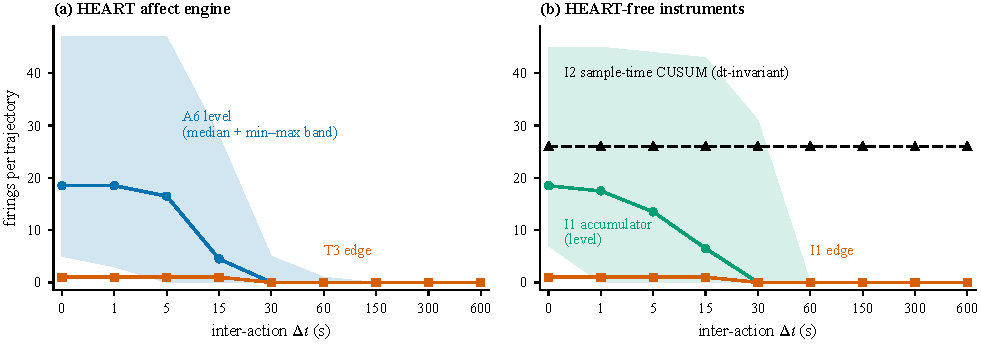
\includegraphics[width=\textwidth]{fig1}
\caption{The thesis in one figure, three monitor archetypes on the same input.
\textbf{(a)} HEART: the A6 level trigger's median fire count (blue) with min--max
band collapses from a constant alarm to silence across the $\Delta t$ grid,
while the T3 edge trigger (orange) is flat at $\le 1$. \textbf{(b)} HEART-free
instruments over the raw error stream: the I1 wall-clock accumulator (green)
shows the same cliff, its edge variant (orange) stays $\le 2$, and the I2
sample-time CUSUM (black, dashed) is exactly $\Delta t$-invariant at 26 fires.
The failure mode lives in the calibration choice, not the state model.
$x$-axis is the discrete $\Delta t$ grid (linear index, labeled in seconds).}
\label{fig:fig1}
\end{figure}

\begin{figure}[t]
\centering
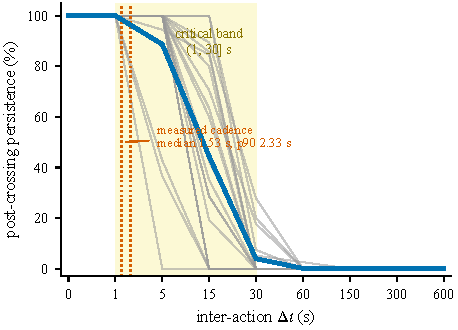
\includegraphics[width=0.62\textwidth]{fig2}
\caption{Post-crossing persistence vs $\Delta t$: 20 thin per-trajectory lines
(grey), mean (blue), with the critical band $(1, 30]$\,s shaded. Measured real
agent cadence (median 1.53\,s, p90 2.33\,s; dotted) sits deep inside the
constant-alarm regime.}
\label{fig:fig2}
\end{figure}

\section{Measured Real Cadence}
\label{sec:cadence}

The sweep's $\Delta t$ is synthetic, and the SWE-bench traces record no
wall-clock times (we verified the submission's public artifacts carry none). We
therefore instrumented a real agent loop directly: a tool-call hook logs an ISO
wall-clock timestamp, tool name, and result status for every action, with zero
interference with the session. Five real debugging runs on cloned open-source
Python repositories (verified bug injection, real test suites; 7--32 actions per
run) yield a pooled $n = 65$ inter-action sample: \textbf{median 1.53\,s, p90
2.33\,s, max 15.87\,s} (the maximum is a full slow test-suite step; test
execution dominates the tail at p90 $= 15.5$\,s by tool type, while reads and
edits sit at 1--2\,s). Only 3.1\% of actions exceed 5\,s; none exceeds 30\,s.
Lag-1 autocorrelation of $\Delta t$ is approximately zero (0.033): heavy steps
did not cluster. An earlier toy probe and token-based reconstructions of the
original traces (medians 1.1--4.4\,s under assumed decode rates) corroborate the
range from independent directions.

Placed on Table~\ref{tab:persistence}'s grid, measured real cadence sits at the
$\Delta t \in [1, 5]$\,s grid points---\textbf{inside the constant-alarm regime
for every trajectory}, with rare transient excursions toward the band's edge
during slow-suite steps. Two consequences. First,~\cite{P1}'s empirical finding
is vindicated: the $\Delta t = 0$ replays approximated the regime real fast
agents actually occupy; the mechanism was wrong, the regime was right. Second,
the dead regime ($\Delta t \ge 60$\,s) is not reached by this workload---but it
is plausibly reached by deployment patterns we did not measure: long
reasoning-model thinking time, CI pipelines, container builds, and human
approval gates routinely exceed 60\,s. We state this as an extrapolation, not a
measurement. The selecting variable is the \textbf{deployment latency profile}:
the same monitor on the same agent behavior is a constant alarm in a fast tool
loop and silent in a human-gated loop. A monitor designer who does not log
inter-action latency cannot know which monitor they have deployed.

\textbf{Measurement limitation, stated plainly:} the instrumented loop used a
small, fast model on small repositories; frontier-model loops with heavy prefill
and long reasoning are slower, so our median is a lower bound for the
deployments of greatest interest---which strengthens the deployment-profile
concern rather than weakening it.

\section{Real Burst Structure: Regimes Are Stable Within a Run}
\label{sec:burst}

Uniform $\Delta t$ leaves open whether realistic non-uniform latency makes the
monitor \emph{flicker}---crossing and re-crossing threshold as heavy steps drain
the state---which would make its firings a latency detector wearing an affect
costume. We tested this with pre-registered conditions per trajectory: C1,
constant $\Delta t$ at the measured median (1.53\,s); C2, i.i.d.\ lognormal
$\Delta t$ fit to the measured distribution (10 seeds); C3, the five real
ordered latency sequences from Section~\ref{sec:cadence}, tiled to trajectory
length with burst structure intact (420 replays total). Pre-registered
hypotheses: H5, the level trigger flickers (median crossing count $> 2$) on
trajectories whose critical interval brackets the median; H6, T3 stays $\le 3$
net fires in all conditions.

\textbf{Disclosure of design timing.} C1--C3 and H5/H6 were committed before
execution; their parameters necessarily derive from Section~\ref{sec:cadence}'s
measurements, as pre-specified. An analytic pre-check (decay from the
frustration clamp to below 0.7 requires ${\sim}88$\,s of silence; the largest
measured gap is 15.9\,s) predicted C1--C3 would not reach the flicker regime.
Rather than over-read the expected null, we added one exploratory
condition---C4, the same real burst sequences time-scaled into each trajectory's
critical band---specified after the pre-check but before any replay was run, and
labeled exploratory throughout. We verified, against the committed
pre-registration document, that the H5/H6 wording and metrics are unchanged from
the version committed before execution, and that only C4 and the
analytic-expectation note were added afterward (see Appendix~\ref{app:prereg}
for the provenance check and its caveat).

\textbf{Results.} H5 is not supported: under C2 and C3, all eligible
trajectories show median crossing counts $\le 1$. Under real ordered bursts
(C3), 19/20 trajectories are clean single-crossing accumulators; the single
exception (a trajectory hovering near 0.7 exactly when the 16\,s heavy step
lands) double-crosses in 3 of 5 sequences---a boundary case, not flicker. Per
the pre-registration's falsification clause, the knife-edge framing is
accordingly softened: within a run, at measured cadence, the regime is stable.
The exploratory C4 supplies the other half: with identical burst \emph{shapes}
shifted into the critical band, 9/20 trajectories multi-cross (up to 4
crossings; flicker index up to 3)---the in-band sensitivity is real, but it is
bounded re-crossing, never wild oscillation. H6 is supported, and beyond its
scope: T3 stays at $\le 1$ net fire in every C1--C3 cell and $\le 3$ even in C4.

Together, Sections~\ref{sec:sweep}--\ref{sec:burst} replace ``latency noise
selects the failure mode'' with the more precise claim the data supports:
\textbf{the regimes are bistable across deployments and stable within them.}
Latency variation inside a fast loop does not toggle the monitor; moving the
deployment's latency profile across the $(1, 30]$\,s band does.

\begin{figure}[t]
\centering
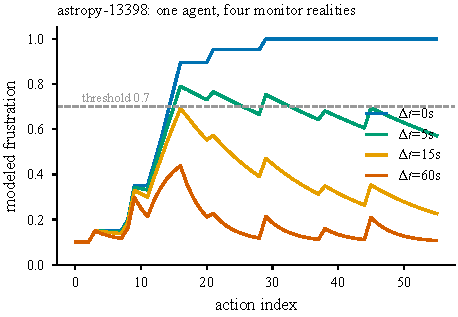
\includegraphics[width=0.62\textwidth]{fig3}
\caption{Frustration vs action index for one trajectory
(\texttt{astropy-13398}) at $\Delta t \in \{0, 5, 15, 60\}$\,s: the same agent
behavior, four monitor realities, from a permanent alarm to a state that never
reaches threshold.}
\label{fig:fig3}
\end{figure}

\section{The Class, Not the Engine}
\label{sec:class}

A natural objection: perhaps the bistability is an artifact of HEART---its 18
dimensions, its heuristic rules, its conflict mechanics. We test the class-level
claim with two minimal instruments over a HEART-independent input: the raw
per-action binary error indicator $e_i$ (verified identical across all
$\Delta t$-variant replays), on the same 20 trajectories and the same
$\Delta t$ grid, with all constants pre-registered.

\textbf{I1, a wall-clock leaky accumulator:}
$s_i = \mathrm{clamp}_{01}(s_{i-1} e^{-\lambda \Delta t} + 0.15\, e_i)$, with
the same half-life as HEART frustration ($\lambda = \ln 2 / 150$) by design,
isolating the calibration choice; level trigger at 0.7, edge trigger with
hysteresis at 0.7/0.5. \textbf{I2, a sample-time CUSUM:}
$g_i = \max(0, g_{i-1} + e_i - 0.10)$, fire at $g \ge 1.0$---by construction
$\Delta t$-free.

\textbf{Results.} I1 reproduces the two-regime structure: the trap holds on
20/20 trajectories at $\Delta t = 0$ (18/19 crossers at $\Delta t = 1$), and the
state never reaches threshold on 20/20 at $\Delta t \ge 60$---the same cliff, on
a one-dimensional accumulator with no emotions, no rules, and no engine. I2 is
exactly invariant: identical fire-index sets at all nine $\Delta t$ values on all
20 trajectories (26 fires throughout, the flat reference line of
Figure~\ref{fig:fig1}). I1's edge trigger fires at most 2 times anywhere. One
pre-registered conjunct failed and is reported as such: we predicted I1's
critical intervals would fall in the same $(1, 30]$ band as HEART's; 16/20 do,
while 4 land in adjacent bins ($(30, 60]$ for three high-error-rate
trajectories, $(0, 1]$ for the sparsest). Per-trajectory critical $\Delta t$s
correlate between instruments at Spearman $\rho = 0.530$. The honest statement:
\textbf{cadence bistability is a property of wall-clock-calibrated leaky
integrators sampled at agent cadence}---the band's exact placement depends on
input stream and step size, within the same order of magnitude. The
error-stream statistics (rates 0.09--0.64) and a step size larger than HEART's
typical realized deltas account for the placement differences.

The three-archetype contrast is the paper in one figure: the wall-clock level
trigger's cliff, the edge trigger's flat $\le 2$ line, and sample-time CUSUM's
exact invariance, all on the identical input stream. The failure mode lives in
the calibration choice, not in any particular state model.

\section{A First-Order Scaling Rule (and Its Limits)}
\label{sec:scaling}

Balancing per-action decay drain against mean per-action event input $r$ at
threshold $\theta$ gives the trap condition
$r \ge (1 - 2^{-\Delta t/T_{1/2}})(\theta - B)$, hence a predicted critical
$\Delta t = -(T_{1/2}/\ln 2)\ln(1 - r/(\theta - B))$ with zero free parameters.
Computed from each trajectory's realized input statistics, predictions land at
5.6--13.4\,s---the right order of magnitude, inside the observed population
band---but only 8/20 fall within their trajectory's interval-censored
observation. An exploratory correction (estimating $r$ from the pre-saturation
region only, motivated by clamp censoring of 0--67\% of input; specified after
seeing the original residuals and labeled as such) repairs the diagnosed
mechanism yet \emph{reduces} interval accuracy to 6/20, trading
under-predictions for over-predictions. We take this as informative failure: a
mean-rate model carries the correct dimensionless structure---input rate
$\times$ half-life vs.\ threshold elevation, the quantity any leaky-integrator
monitor designer should compute---but per-trajectory transitions are governed by
input burstiness that a mean rate cannot express. We deliberately stop here
rather than fit burst-aware parameters post hoc.

\begin{figure}[t]
\centering
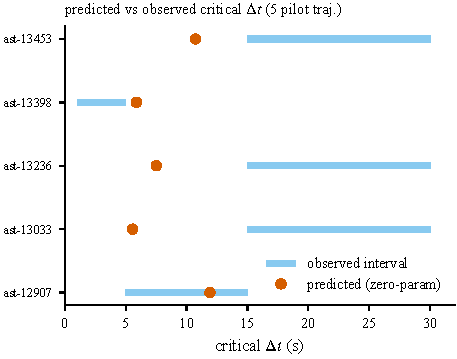
\includegraphics[width=0.62\textwidth]{fig4}
\caption{Zero-parameter predicted critical $\Delta t$ (orange points) against
interval-censored observations (blue bars) for the 5 pilot trajectories: right
order of magnitude, but only a minority land inside their interval.}
\label{fig:fig4}
\end{figure}

\section{Transition Triggers Escape the Trap but Not the Timing Problem}
\label{sec:transition}

We pre-registered four transition-aware triggers over the same frozen state
stream: T1 velocity (windowed first difference $\ge 0.5$ on the 5-emotion
negative sum), T2 acceleration (second difference $\ge 0.3$), T3 rising-edge
saturation entry (fires on upward crossing of the identical 0.7 frustration
threshold; re-arms below 0.5), T4 plateau-no-recovery, all behind a 5-action
refractory wrapper, thresholds fixed before any result existed.

\textbf{Saturation escape (pre-registered H1): partially confirmed, cleanly for
T3.} Across the $n = 20$ set, the full uniform grid, all non-uniform conditions
including exploratory C4, and the HEART-free instrument of
Section~\ref{sec:class}, edge detection fires 0--3 times per trajectory, at
saturation onset (re-fires only when decay legitimately pulls the state below
the hysteresis floor and it re-crosses). At $\Delta t = 0$, where A6 fires on
18--82\% of actions, T3 fires once. Since T3 and A6 share the exact threshold
value, the comparison isolates level- vs.\ edge-detection: the entire pathology
of A6 is the \emph{level} primitive, not the threshold, the emotion model, or
the data. T1 mostly escapes (post-saturation fire rate 2--27\%); T2 never fires
anywhere---its pre-registered second-difference threshold is mis-scaled to the
engine's per-event delta magnitudes (0.05--0.2), a calibration lesson we report
rather than repair; T4 degenerates (26--88\% of post-saturation actions),
confirming that plateau detection at saturation reproduces the level trigger's
failure with extra steps.

\textbf{Live operation.} The instrumented loop of Section~\ref{sec:cadence} also
ran the frozen engine and T3 online with real elapsed $\Delta t$. On the
32-action run, T3 fired exactly once, at the rising edge (frustration
$0.603 \to 0.750$), while A6 was true on 25 of 32 actions---the level-vs-edge
contrast in a single live log (Figure~\ref{fig:fig5}).

\begin{figure}[t]
\centering
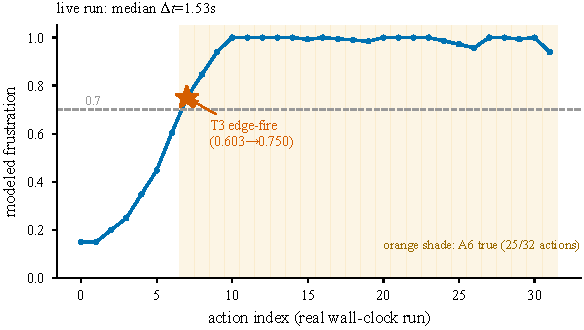
\includegraphics[width=0.7\textwidth]{fig5}
\caption{Live instrumented run (real wall-clock $\Delta t$, median 1.53\,s):
modeled frustration ramps from 0.10 to saturation; T3 fires once at the rising
edge (star, $0.603 \to 0.750$) while A6 is true on 25 of 32 actions (orange
shading)---the level-vs-edge contrast in live operation.}
\label{fig:fig5}
\end{figure}

\textbf{Timing alignment (pre-registered H2): failed, as the pre-registration's
falsification clause anticipated.} On the one human-labeled trajectory, the
transition triggers' net firings overlap the $\ge 2$-annotator consensus set at
2/9, and both hits come from the degenerate T4 surviving an arbitrary refractory
subsample---a stopped-clock effect we decline to count as alignment. Given
\cite{P1}'s central finding that three trained annotators agree on intervention
points only marginally above chance (location $\alpha = +0.047$), this is the
coherent outcome: transition triggers repair the \emph{detector}; nothing can
repair an unreliable \emph{target}. Solving saturation and solving timing are
different problems, and only the first is solved here.

\section{Related Work}
\label{sec:related}

\textbf{Runtime oversight of agents.}
A growing line of work interrupts an agent by checking its trajectory against
safety conditions. AgentSpec~\cite{agentspec} compiles user-specified rules
(trigger--predicate--enforce) and fires when a predicate matches the current
action; AgentHarm~\cite{agentharm} benchmarks harmful agent behavior that such
monitors aim to catch. These systems threshold per-action predicates rather
than an accumulated, time-decayed statistic, and so lie outside the
leaky-integrator class our result concerns. ProbGuard~\cite{probguard} is the
closest in spirit---it predicts the probability of reaching an unsafe state and
intervenes when that probability crosses a threshold---but the quantity it
thresholds is an \emph{instantaneous} predicted probability recomputed from the
current symbolic state at each step, not a statistic that integrates past
evidence with a wall-clock decay. It is therefore also outside our class: it
has no half-life to mis-calibrate against cadence, and our bistability result
does not apply to it. Our prior work~\cite{P1} is the wall-clock-calibrated
member whose failure this paper dissects.

\textbf{Sequential change detection.}
The classical home of edge-versus-level detection is the cumulative-sum chart
of Page~\cite{page1954}, with asymptotic optimality established by
Lorden~\cite{lorden1971} and the modern landscape surveyed by Truong et
al.~\cite{truong2020}. CUSUM is defined in \emph{sample time}---its drift term
is subtracted once per observation---which is exactly why our Section~7 control
(I2) is cadence-invariant: it is classical CUSUM behaving classically. We claim
no novelty for edge detection or for CUSUM; the contribution is the
\emph{calibration-mismatch} analysis that separates sample-time from
wall-clock-time dynamics at \emph{agent} cadence, where inter-action intervals
vary across deployments by orders of magnitude. The two-threshold hysteresis
our T3 trigger uses is the Schmitt trigger~\cite{schmitt1938}, the canonical
bistable detector with separate set/reset levels.

\textbf{Calibrated-decay monitors and label variation.}
Wall-clock-calibrated leaky integrators---exponential-moving-average behavioral
baselines and drift statistics with fixed half-lives---are common in production
agent and service monitoring; they are precisely the family our analysis places
at risk when the sampling cadence is not the cadence the half-life was tuned
for. Finally, our evaluation of whether any trigger \emph{recovers human
intervention timing} inherits the framing of LLM-as-judge
evaluation~\cite{zheng2023} and of human label
variation~\cite{plank2022,krippendorff2004}: as in~\cite{P1}, the target itself
is a low-reliability construct, so repairing the detector (Section~9) does not,
and cannot, repair the target.


\section{Limitations}
\label{sec:limitations}

Synthetic uniform $\Delta t$ in Section~\ref{sec:sweep} (bounded by
Sections~\ref{sec:cadence}--\ref{sec:burst}'s measured and replayed real timing,
but the SWE-bench traces' own timing remains unrecoverable); measured cadence
from a small-model loop on small repos (a lower bound for frontier loops---the
deployments most likely to enter the transition band are exactly the ones not
measured); the dead-regime claim for slow deployments is an extrapolation from
the sweep, not a measurement; one harness format and one model family's traces;
the class-level demonstration uses one additional instrument over one input
stream (binary errors)---broader instrument and stream coverage would strengthen
it, and the band's placement is instrument-dependent (one pre-registered band
conjunct failed, reported in Section~\ref{sec:class}); timing-alignment
evaluation rests on one labeled trajectory pending expanded annotation; the
scaling rule is order-of-magnitude only; T2/T4 show that pre-registration
without pilot calibration risks degenerate cells, a cost of the no-tuning
discipline we accept; C4 is exploratory and its in-band flicker result awaits
confirmatory replication.

\section{Conclusion}
\label{sec:conclusion}

A wall-clock-calibrated leaky-integrator monitor has no cadence regime in which
it detects moments on agent streams: below the critical band it is a constant
alarm, above it it is dead, the regimes are stable within a run, and the
transition band sits where real deployments live---so the deployment's latency
profile, a quantity monitor designers neither control nor typically log,
silently selects which failure is deployed. The structure is a property of the
calibration class: a one-dimensional accumulator over raw errors shows the same
cliff, while a sample-time CUSUM over the identical stream is exactly
cadence-invariant. Measured real agent cadence (median 1.53\,s) sits firmly in
the constant-alarm regime, vindicating the empirical content of our earlier
report under a corrected mechanism. The correct primitive at any cadence is
transition detection---a rising edge with hysteresis fired 0--3 times per
trajectory in every condition tested, including live operation---but detecting
transitions is not the same as timing interventions, which remains a
low-reliability human construct. We arrived here by auditing our own published
pipeline, finding its decay term inert, and pre-registering the counterfactuals
the flaw made possible; we commend the genre.


\bibliographystyle{plainnat}
\bibliography{references}

\appendix
\section{Appendix}

\subsection{Trajectory selection}
15 selected, 11 skipped for length, 0 parse failures (first 15 by instance id
with 25--70 actions that parse cleanly, excluding the 5 pilot trajectories).
Full skip log released with the artifacts.

\subsection{Per-trajectory tables}
Full saturation table ($\Delta t = 0$), per-trajectory critical-$\Delta t$
intervals, and zero-signal coverage are released as
\texttt{SCALE\_REPORT.md} and the \texttt{fig\_data/} CSVs.

\subsection{Pre-registration provenance and hypothesis scorecard}
\label{app:prereg}
Pre-registration documents for all phases are released verbatim
(\texttt{PREREGISTRATION\_PHASE7.md}, \texttt{PREREGISTRATION\_PHASE8.md}).
Full hypothesis scorecard: H1 partial (T3 yes; T1 borderline; T2 vacuous; T4
no), H2 failed, H3 superseded by the $\Delta t$ audit, H4 pending annotation, H5
not supported (with the C4 exploratory complement), H6 supported, H7 partial
(two-regime supported; strict band conjunct failed 16/20), H8 supported (exact
invariance 20/20), H9 supported (max 2).

\paragraph{Provenance check for the Section~\ref{sec:burst} disclosure (resolving
the draft's \texttt{[CONFIRM]} marker).} The released
\texttt{PREREGISTRATION\_PHASE7.md} states H5 and H6 verbatim as ``\emph{H5:
under C2/C3, A6 exhibits flicker (median crossing count $>2$) on trajectories
whose uniform-$\Delta t$ critical interval brackets the $\Delta t$ median}'' and
``\emph{H6: T3 net fire count remains $\le 3$ under all conditions},'' which are
exactly the hypotheses scored in \texttt{NONUNIFORM\_REPORT.md}; C4 and the
``analytic expectation'' subsection are present as a separately labeled
\emph{exploratory} block. \textbf{Caveat for the author:} the artifact tree was
\emph{not} under version control during the study, so a git diff of this file
does not exist. The evidence supporting ``unchanged before execution'' is
therefore (i) the file's text matches the report's scored wording exactly, and
(ii) filesystem modification times order the pre-registration
(\texttt{2026-06-10 21:26}) before the results report
(\texttt{2026-06-10 21:30}). The draft's phrase ``git-timestamped'' in
Section~\ref{sec:setup} should be softened to ``timestamped'' (or the repository
placed under git and the prereg commits cited) before submission, since
filesystem mtimes are weaker provenance than signed commits.

\subsection{Scaling rule}
Derivation and both estimators (full-trajectory $r$ and pre-saturation $r$),
with censoring diagnostics, in \texttt{ANALYTIC\_DT\_REPORT.md}.

\subsection{$\Delta t$ audit}
Code-path trace with line references and the erratum text in
\texttt{DT\_AUDIT.md}.

\subsection{Instrumentation}
Hook design, tool-name mapping table, and converter limitations (empty
thoughts; A9 reasoning-feature triggers inapplicable to hook traces); timing
distributions per run and per tool type in \texttt{data/live\_runs/}.

\subsection{Non-uniform replay}
Condition construction, seeds, per-condition tables, and the boundary case in
\texttt{NONUNIFORM\_REPORT.md}.

\subsection{Generality instruments}
Error-stream statistics per trajectory, I1/I2 definitions and unit tests, full
Tables A--D, and the Spearman computation in \texttt{GENERALITY\_REPORT.md}.


\end{document}
